\subsection{Entity Typing} \label{entity_typing}
\subsubsection{Overview}
Entity Typing (ET) is a subtask of Named Entity Recognition (NER) originally proposed in the 90s~\cite{MUC6}. ET aims to assign types\footnote{synonyms that could be used in this work: labels, classes} from a type set to named entities appearing in a text. Given a type set $T$, a sentence $S = c_{L} + m + c_{R} $ where $m$ is the mention span and $c_{L/R}$ is the left/right context, the goal of ET is to predict the correct types $t_{m} \subseteq T $ that better describe $m$ with respect to $S$. Since $t_{m}$ may contain multiple types, the ET task is considered a multiclass multilabel classification problem~\cite{lopez2020fully}.

Figure~\ref{fig:et_pipeline} shows the steps involved in a generic problem of ET. The input sentence requires to classify the mention of ``George Washington" with respect to the given context. Before feeding any machine learning model, the text must be transformed into a machine-readable format. This step can be based on the extraction of handcrafted features or, for most approaches from recent years can rely on newer encoding strategies ranging from Word2Vec to BERT. Finally, the preprocessed input is provided to the model that produces an output vector containing the predictions for each type in $T$. Depending on the adopted model, ET approaches can be grouped into two main categories: classification approaches like~\cite{yosef-etal-2012-hyena, Ling2012FineGrainedER, shimaoka2016attentive, choi, xu-barbosa-2018-neural}, or regression approaches like~\cite{yogatama-etal-2015-embedding, abhishek-etal-2017-fine, lopez-etal-2019-fine, ren-etal-2016-afet}.

\begin{figure}[H]
    \centering
    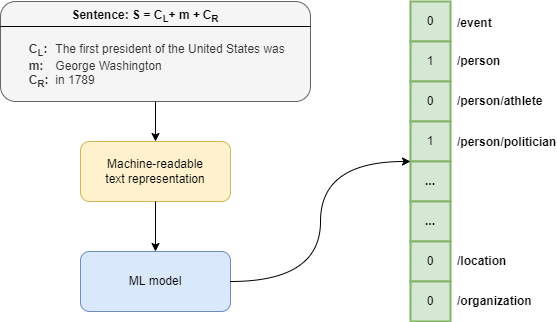
\includegraphics[width=.8\linewidth]{figures/et_pipeline.png}
    \caption{ Entity typing pipeline }
    \label{fig:et_pipeline}
\end{figure}

Using ET to detect the semantic classes of named entities can be beneficial for several NLP applications such as Question Answering, Knowledge Base Population, Relation Extraction, Entity Linking, and many others. Sometimes, the context of an NLP application requires dealing with very specific types, thus needing the extension of the typical type set composed of \verb|Person|, \verb|Organization| and \verb|Location|. For this reason, several datasets with larger type sets have been proposed over the years and used to evaluate such tasks~\cite{Ling2012FineGrainedER, ren2016noise, choi, ontonotes}. When the type set has a high cardinality, the ET task takes the name of Fine-Grained Entity Typing (FET). The type set of a FET dataset is usually organized in a hierarchical way, where the relations between coarse types and fine-grained types are represented by the edges of a tree. Each coarse type can be seen as the root node of a tree. Regarding the fine-grained types, they are represented as the descendants of the root: the deeper the node, the finer the type. The relations expressed by these hierarchical trees are the type dependencies we want to exploit in this thesis using Neural-Symbolic Integration.

\subsubsection{Approaches that exploit hierarchical information}
% specialized models
As discussed in the introduction, exploiting the hierarchy is a technique used by different approaches to face FET tasks. In~\cite{rahman2010} a model is trained to predict one branch of the hierarchy and one model per branch is trained to specialize the classification, obtaining 30 models. Similarly,~\cite{yosef-etal-2012-hyena} defines a classifier for each type and uses them following the hierarchy in a top-down manner. 

% logit filtering techniques based on hierarchy
\cite{yogatama-etal-2015-embedding,ma-etal-2016-label,ren-etal-2016-afet} defines a single classifier for all types, but filter the predictions using the hierarchy in a top-down manner, filtering out the types that are not descendants of already predicted types. The differences between these approaches reside in the inference technique:~\cite{yogatama-etal-2015-embedding} uses a fixed threshold; ~\cite{ma-etal-2016-label} a relative threshold;~\cite{ren-etal-2016-afet} infers the type with the maximum logit along with its brothers, then processes the sons of the inferred type until the bottom of the hierarchy is reached or the maximum is lower than a fixed threshold. The inference method of ~\cite{ren-etal-2016-afet} is used also by~\cite{abhishek-etal-2017-fine,ren2020FETHI}.

% hierarchy in the model/optimization
\cite{ma-etal-2016-label,ren-etal-2016-afet,shimaoka2016neural,murty-etal-2018-hierarchical,xu-barbosa-2018-neural,lopez-etal-2019-fine,wu2019,ren2020FETHI,chen-etal-2020-hierarchical} inject hierarchical information in the model through type representation and/or optimization techniques.~\cite{ma-etal-2016-label,shimaoka2016neural} represent each type through a one-hot vector with values $1$ for the type and for its ancestors.~\cite{ren-etal-2016-afet,wu2019} use hierarchy to derive similarities between types, thus weighting the errors.~\cite{murty-etal-2018-hierarchical} represent each type with a vector obtained with Rescal~\cite{Nickel2011Rescal} or ComplEx~\cite{trouillon2016complex}, thus injecting also hierarchical information about types.~\cite{xu-barbosa-2018-neural} boost the prediction of a node based on its ancestors.~\cite{lopez-etal-2019-fine,ren2020FETHI} use a layer to predict types for each level in the hierarchy, then each layer uses the higher level prediction as input.~\cite{chen-etal-2020-hierarchical} use the hierarchy to select hard negatives for a learning-to-rank training technique.

Details on how hierarchical rules are exploited in this work will be described in section~\ref{knowledge_generation}.

\subsubsection{Approaches based on BERT}
In the architecture of a FET network, the encoding of the entity mention within its context is a central characteristic of each approach. Since in our architecture BERT is central for the encoder, we now focus on the approaches that use BERT or derived language models as encoder.~\cite{wang2020} tested different contextual encoders by fixing an architecture and showed that BERT-based encoders achieved better performance in FET. Similarly,~\cite{dai-etal-2020-semantic-relations,liu-etal-2021-fine,onoe-etal-2021-modeling} use BERT as encoder to obtain a contextual vector from the input mention within its context.~\cite{dai-etal-2021-ultra} use BERT to obtain types by masking the entity mention in the input sentence and optimizing the generated tokens to obtain the tokens that represent the correct types. Finally, ~\cite{Hou2021} uses an ensemble encoder comprising SpanBERT~\cite{joshi-etal-2020-spanbert}.

Details on the FET network architecture designed for the experiments of this thesis will be presented in sections~\ref{baseline_model}.
